\documentclass[a4paper,11pt,twoside]{article}

\usepackage{palatino,newtxmath,bbold}	%% Písma
\usepackage{microtype}					%% Lepší mezery
\usepackage[T1]{fontenc}
\usepackage[utf8]{inputenc}	            %% Kódování textu
\usepackage[czech]{babel}               %% České nápisy
\usepackage{amsfonts,amsmath}			%% Matematické symboly (amssymb koliduje s jiným balíkem)

\usepackage{epsfig}                     %% Obrázky
\usepackage[subrefformat=simple,labelformat=simple]{subcaption} %% Podobrázky
\usepackage{graphicx}					%% Doplňující příkazy pro obrázky

\usepackage{xifthen}					%% Podmínka if - then
\usepackage{makeidx}					%% Rejstřík
%\usepackage{showframe}
%\usepackage{showidx}

\usepackage[multiple]{footmisc}			%% Lepší formátování poznámek pod čarou - nefunguje s hyperref
%\usepackage{fnpct}						%% Lepší formátování poznámek pod čarou
\usepackage{comment}					%% Komentáře
\usepackage{scrextend}					%% Vylepšené formátování (addmargin)
\usepackage{xcolor}						%% Barvy
\usepackage{indentfirst}				%% Odsazení prvního odstavce
\usepackage{fancyhdr}
\usepackage{blkarray}					%% Pro komentované vektory
\usepackage{empheq}                     %% Box around equations

\usepackage{csquotes}
\usepackage{expl3}						%% Jinak nefunguje biblatex
\usepackage{biblatex}
\addbibresource{S:/Fyzika/Bibliography/References.bib}

%\bibliographystyle{phaip}

\graphicspath{{figures/}}

%\usepackage{showlabels}                 %% Temporarily show the names of labels
%\renewcommand{\showlabelfont}{\tiny\bfseries\color{black}}

\usepackage{mathtools}
%\mathtoolsset{showonlyrefs}            %% Remove equation number of unrefferenced equations

\usepackage[unicode]{hyperref}			%% Hypertextové odkazy
\hypersetup{
	pdftitle={Cvičení k přednášce Atomová fyzika (NFUF301)},
	pdfauthor={Pavel Stránský},
	pdffitwindow=true,
	colorlinks=true,
	urlcolor=cyan,            			%barva textu pri tisku
	linkcolor=red,
	citecolor=green,
	filecolor=magenta
}

% Velikost stránky
\addtolength{\topmargin}{-1.5cm} %\addtolength{\textheight}{-10cm}
\addtolength{\textwidth}{4cm} \addtolength{\textheight}{4cm} % Šířka a výška textu
\addtolength{\voffset}{-0.5cm} % Horní okraj
\addtolength{\hoffset}{-2cm}
\setlength{\headheight}{15pt}

\pagestyle{fancy}

% Definice
\DeclareMathOperator{\e}{e}
\DeclareMathOperator{\tg}{tg}
\DeclareMathOperator{\cotg}{cotg}
\DeclareMathOperator{\arccotg}{arccotg}
\DeclareMathOperator{\sign}{sign}
\DeclareMathOperator{\arccosh}{arccosh}
\DeclareMathOperator{\arcsinh}{arcsinh}
\DeclareMathOperator{\divergence}{div}
\DeclareMathOperator{\gradient}{grad}
\DeclareMathOperator{\trace}{Tr}
\DeclareMathOperator{\real}{Re}
\DeclareMathOperator{\imaginary}{Im}
\DeclareMathOperator{\Ai}{Ai}
\DeclareMathOperator{\Bi}{Bi}
\DeclareMathOperator{\Tp}{\mathsf{T}}

\renewcommand{\d}{\mathrm{d}}
\newcommand{\D}{\mathcal{D}}

\def\O#1{\mathcal{O}\left({#1}\right)}

\def\ket#1{\left|{#1}\right\rangle}
\def\bra#1{\left\langle{#1}\right|}
\def\mean#1{\left\langle{#1}\right\rangle}
\def\braket#1#2{\left\langle{#1}\middle|{#2}\right\rangle}
\def\matrixelement#1#2#3{\left\langle{#1}\middle|{#2}\middle|{#3}\right\rangle}
\def\ketbra#1#2{\left|{#1}\middle\rangle\middle\langle{#2}\right|}
\def\projector#1{\left|{#1}\middle\rangle\middle\langle{#1}\right|}

\def\unit#1{\,\mathrm{{#1}}}
\def\c{,\!}

\def\hi#1{^{({#1})}}

\def\clebsch#1#2#3#4#5#6{\mathcal{C}^{#5\,#6}_{#1\,#2\:#3\,#4}}
\def\threej#1#2#3#4#5#6{\begin{pmatrix}#1&#2&#3\\#4&#5&#6\end{pmatrix}}

\def\commutator#1#2{\left[{#1},{#2}\right]}
\def\associator#1#2#3{\left[{#1},{#2},{#3}\right]}

\def\abs#1{\left|{#1}\right|}
\def\abss#1{\left|{#1}\right|^{2}}							% Square of the absolute value
\def\intinf{\int_{-\infty}^{\infty}}						% Infinite integral

\def\minus#1{\left(-1\right)^{#1}}
%\def\ui#1{(#1)}
\def\ti#1{\mathrm{#1}}										% Text index

\def\error#1{{\color{red}{\bf{#1}}}}
\def\trick#1{{\color{blue}#1}}

\def\hilbert#1{\mathcal{#1}}								% Hilbert space
\def\group#1{\mathrm{#1}}									% Group
\def\algebra#1{\mathrm{#1}}

\def\vector#1{\boldsymbol{#1}}								% Vector
\def\matrix#1{\mathsf{#1}}										% Matrix
\def\axis#1{\mathrm{#1}}

\def\2F1#1#2#3#4{\,{}_{2}F_{1}\!\left(#1,#2,#3;#4\right)}
\def\1F1#1#2#3{\,{}_{1}F_{1}\!\left(#1,#2;#3\right)}

\def\operator#1{\mathsf{\hat{#1}}}
\def\vectoroperator#1{\boldsymbol{\mathsf{\hat{#1}}}}
\def\tensoroperator#1#2{\hat{\mathbb{#1}}^{(#2)}}					% tensor operator
\def\tensoroperatorcomponent#1#2#3{\hat{\mathsf{#1}}^{(#2)}_{#3}}	% tensor operator - component
\def\reducedmatrixelement#1#2#3{\left(#1\middle\lVert#2\middle\rVert#3\right)}	    % Reduced matrix element

\def\propagator{G(\vx_{\rf},t_{\rf};\vx_{\ri},t_{\ri})}

\newcommand{\partialderivative}[3][]{\ifthenelse{\isempty{#1}}	% Partial derivative
	{\frac{\partial{#2}}{\partial{#3}}}
	{\frac{\partial^{#1}{#2}}{\partial{#3}^{#1}}}
}

\newcommand{\derivative}[3][]{\ifthenelse{\isempty{#1}}	% Normal derivative
	{\frac{\d{#2}}{\d{#3}}}
	{\frac{\d^{#1}{#2}}{\d{#3}^{#1}}}
}

\def\conjugate#1{{#1}^{\dagger}}
\def\transpose#1{{#1}^{\intercal}}

\def\operatorconjugate#1{\conjugate{\operator{#1}}}

\def\makematrix#1{\begin{pmatrix}#1\end{pmatrix}}       % Matrix
\def\Vdots{\vphantom{0}\smash[t]{\vdots}}

\def\equationcomment#1{\begin{vmatrix}#1\end{vmatrix}}  % Comment in equation (e.g. substitution in integral)

\long\def\important#1{\boxed{#1}}

\def\MeV{\mathrm{MeV}}
\def\im{\mathrm{i}}
\def\const{\mathrm{const}}

\includecomment{theory}
%\excludecomment{solution}
%\includecomment{note}

% Homework - části, které jsou (byly) za domácí úkol, a proto by se neměly vyskytnout ve sbírce
%\excludecomment{homework}

% homeworknote - části, které jsou navázané na řešení; část s domácím úkolem; vzájemně exklusivní s prostředním homework
\newenvironment{homeworknote}{}{}

% Toto se odkomentuje pro tištěnou kompletní sbírku
%\excludecomment{homeworknote}
\newenvironment{homework}{}{}

% solution - část s řešením
%\excludecomment{solution}
%\excludecomment{theory}
\newenvironment{solution}{\begin{addmargin}{0.5cm}\color{gray}\subsubsection*{Řešení:}\small}{\end{addmargin}\vspace*{0.3cm}}

\newenvironment{example}{\textbf{\textit{Příklad:}}}{}

\newenvironment{note}[1][]{\vspace*{0.2cm}\noindent\textbf{\textit{\ifthenelse{\isempty{#1}}{Poznámka: }{#1}}}}{}
%\newenvironment{theory}{}{}

\def\sec#1{\subsubsection*{#1}}
\def\sfootnote#1{\footnote{\color{gray}#1}}
\def\scaption#1{\caption{\small\color{gray}#1}}
\def\scaptionx#1#2{\caption[#1]{\small\color{gray}#2}}

\newcommand{\np}{\clearpage\newpage}
%\newcommand{\np}{\clearpage\setcounter{page}{1}\newpage}
%\newcommand{\np}{}\newcommand{\minput}[1]{\input{#1}}

\newcommand{\exercise}[2][]{\ifthenelse{\isempty{#1}}
	{\np\thispagestyle{empty}\subsubsection*{Domácí úkol -- #2}}
	{\np\thispagestyle{empty}\np\subsubsection*{Domácí úkol -- #2 \small{\it{(termín odevzdání: {#1})}}}}
}

\makeindex

\begin{document}

\makeatletter
\@addtoreset{equation}{subsection}
\renewcommand{\theequation}{\arabic{section}.\arabic{subsection}.\arabic{equation}}
%\renewcommand{\thepage}{\arabic{section}.\arabic{page}}
%\@addtoreset{page}{section}
\makeatother

\title{Cvičení k přednášce Atomová fyzika (NFUF301)}
\date{\today}
\author{Pavel Stránský}

\maketitle
\pdfbookmark{\contentsname}{Contents}
\tableofcontents\np

\section{Černé těleso}
\subsection{Rayleighův-Jeansův zákon}
    Odvoďte objemovou hustotu energie černého tělesa pro frekvenci $\nu$ a vlnovou délku $\lambda$.
    Předpokládejte, že energie jednotlivých módů elektromagnetického záření může nabývat jakýchkoliv hodnot.

\subsection{Planckův zákon}
    Odvoďte objemovou hustotu energie černého tělesa za předpokladu, že energie jednotlivých energie módů elektromagnetického záření může nabývat jen celočíselných násobků frekvence módů $\nu$,\footnote{
        Vztah lze ekvivalentně zapsat pomocí úhlové frekvence $\omega$ a redukované Planckovy konstanty $\hbar$ jako
        \begin{equation}
            E_{n}=\hbar\omega n
        \end{equation}
    }
    \begin{equation*}
        E_{n}=h\nu n,
    \end{equation*}
    kde $n$ je přirozené číslo a $h$ je konstanta (Planckova konstanta).

\subsection{Wienův posunovací zákon}
    Odvoďte, pro jakou frekvenci a pro jakou vlnovou délku je objemová hustota energie černého tělesa daná Planckovým zákonem maximální.

\subsection{Stefanův-Boltzmannův zákon}
    Odvoďte celkový zářivý výkon černého tělesa o teplotě $T$.

\subsection{Slunce}
    Je-li Slunce v zenitu, je intenzita slunečního záření dopadající na Zemi $I_{\oplus}=1367\unit{Wm^{-2}}$.
    Za předpokladu, že vyzařování Slunce lze považovat za záření černého tělesa, a znáte-li poloměr Slunce $R_{\odot}$ a vzdálenost Země od Slunce $d$, určete teplotu na povchu Slunce.

\subsection{Žárovka}
    Wolframové vlákno v klasické žárovce se rozžhaví na teplotu $T=4000\unit{K}$.
    Jaké procento vyzařované energie je ve viditelné části spektra mezi vlnovými délkami $\lambda\in[380\unit{nm},750\unit{nm}]$?

\subsection{Hlava}
    Odhadněte celkový zářivý výkon holé lidské hlavy bez pokrývky.
    Jaký je rozdíl zářivého výkonu a zářivého příkonu v prostředí, které má $t_{\text{okolí}}=0\unit{^\circ C}$?
    Bazální metabolismus dospělého člověka je přibližně $P_{B}=1700\unit{kcal\,den^{-1}}$.
    Určete, jaké procento energie získané metabolismem se v chladném počasí ztratí hlavou vyzařováním.\footnote{
        Proto je dobré nosit v zimě čepici.
    }

\subsection{Fotonová plachetnice}
    Určete, jaká síla by díky slunečnímu záření působila na čtvercovou plachtu o rozměru $100\unit{m}\times 100\unit{m}$, nacházející se ve vzdálenosti Země. 
    Jak musí být plachta orientovaná, aby síla byla co největší?
    Je síla větší, když plachta záření pohltí, nebo když ho odrazí?

\subsection{Vlákno žárovky}
    Odhadněte délku a poloměr wolframového vlákna žárovky s příkonem $P=100\unit{W}$, víte-li, že teplota vlákna je $T=2700\unit{K}$.\np
\section{Částicový charakter elektromagnetického záření}
    \subsection{Comptonův rozptyl}
        Odvoďte vztah pro energii fotonu $E'_{\gamma}$ a jeho vlnovou délku $\lambda'$, který se rozptýlil na elektronu na úhel $\theta$ (obrázek~\ref{fig:Compton}).
        Energie a vlnová délka fotonu před rozptylem je $E_{\gamma}$ a $\lambda$.
        Předpokládejte, že před rozptylem je elektron v klidu.
        Hmotnost elektronu je $m_{e}$.

        \begin{figure}[!h]
            \centering
            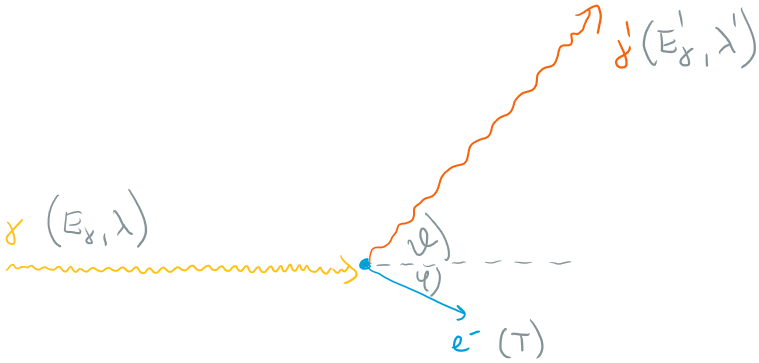
\includegraphics[width=0.6\linewidth]{Compton.png}
            \caption{Comptonův rozptyl fotonu $\gamma$ na elektronu $e^{-}$.}
            \label{fig:Compton}
        \end{figure}

    \subsection{Comptonova vlnová délka}
        Vyjádřete vztah pro změnu vlnové délky fotonu při Comptonově rozptylu $\Delta\lambda=\lambda'-\lambda$ pomocí Comptonovy vlnové délky $\lambda_{c}=h/(m_{e}c)$, kde $h$ je Planckova konstanta, $m_{e}$ hmotnost elektronu a $c$ rychlost světla.

    \subsection{Úhel vylétávajícího elektronu}
        Odvoďte vztah pro úhel $\varphi$, pod kterým vylétá elektron po Comptonově rozptylu (obrázek~\ref{fig:Compton}).

    \subsection{Spektrum $\gamma$ při měření v detektoru}
        \begin{figure}[!h]
            \centering
            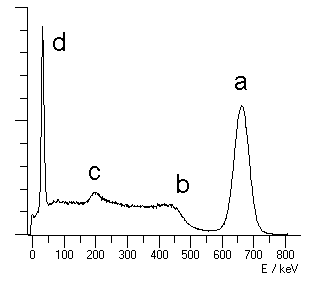
\includegraphics[width=0.35\linewidth]{ComptonSpectrum.png}
            \caption{Detekované Comptonovské spektrum monochromatického $\gamma$ záření.}
            \label{fig:ComptonSpectrum}
        \end{figure}        
    
        Detektor vysokoenergetických kvant $\gamma$ funguje na principu Comptonova rozptylu, kdy kinetická energie rozptýlených elektronů vytvoří impuls elektrického proudu, který se následně zesílí a změří.

        Předpokládejte, že na detektor dopadá monochromatické záření s energií kvant $E_{\gamma}$ vzniklé rozpadem radioaktivního nuklidu.
        Vysvětlete body a, b, c z obrázku~\ref{fig:ComptonSpectrum}; obrázek zobrazuje četnost, se kterou byla detektorem naměřena energie elektronu $E$. 
        Odhadněte, jaká byla energie $E_{\gamma}$, a z této \href{https://cds.cern.ch/record/1309915/files/978-3-642-02586-0_BookBackMatter.pdf}{tabulky} určete nuklid, jehož rozpad je měřen.

        % Zdroj tabulky: https://www.ld-didactic.de/software/524221en/Content/Appendix/ComptonSpectrum.htm\np
\section{Práh reakce}
\subsection{Greisenův-Zatsepinův-Kuzminův limit}
    GZK limit je prahová hodnota energie kosmického protonového záření, nad kterou dojde k interakci protonu s fotonem reliktního záření za vzniku buď protonu a neutrálního pionu, nebo neutronu a kladně nabitého pionu,\footnote{
        K reakci dochází přes $\Delta^{+}$ rezonanci.
    }
    \begin{subequations}
        \begin{align}
            p^{+}+\gamma_{\mathrm{RZ}}
                &\longrightarrow p^{+}+\pi^{0},\\
                &\longrightarrow n^{0}+\pi^{+},
        \end{align}        
    \end{subequations}
    čímž vysokonenergetický foton ztratí energii (je zbržděn).
    Odbvoďte tento limit pro obě reakce.
\np
\section{Rozptyl}
\subsection{Srážkový parametr a diferenciální účinný průřez}
    Odvoďte vztah mezi srážkovým parametrem $b(\theta)$ a diferenciálním účinným průřezem $\derivative{\sigma}{\Omega}$.

\subsection{Rutherfordův rozptyl}
    Vztah pro srážkový parametr u Rutherfordova rozptylu (rozptyl $\alpha$ částice na jádru s protonovým číslem $Z$) na úhel $\theta$ je
    \begin{equation}
        b(\theta)=\frac{d_{0}}{2}\frac{1}{\tg{\frac{\theta}{2}}},
    \end{equation}
    kde
    \begin{equation}
        d_{0}=\frac{2Ze^{2}}{4\pi\epsilon_{0}}\frac{1}{T}
    \end{equation}
    je~\emph{Sommerfeldův parametr} (vzdálenost nejbližšího přiblížení rozptylující a rozptylované částice) a $T$ je kinetická energie $\alpha$ částice v laboratorní soustavě.

    Odvoďte výraz pro diferenciální účinný průřez.

\subsection{Rozptyl na tvrdé kouli}
    \begin{enumerate}
        \item Odvoďte vztah mezi srážkovým parametrem a rozptylem na úhel $\theta$ pro tvrdou kouli.
        \item Odvoďte výraz pro diferenciální účinný průřez.
        \item Určete celkový účinný průřez.
    \end{enumerate}\np

\printindex

%\bibliography{Z:/Share/Fyzika/Bibliography/References.bib}
\printbibliography
%\input{refs}

\end{document}
